\documentclass[journal]{IEEEtran}
\usepackage[a5paper, margin=10mm]{geometry}
%\usepackage{lmodern} % Ensure lmodern is loaded for pdflatex
\usepackage{tfrupee} % Include tfrupee package


\setlength{\headheight}{1cm} % Set the height of the header box
\setlength{\headsep}{0mm}     % Set the distance between the header box and the top of the text


%\usepackage[a5paper, top=10mm, bottom=10mm, left=10mm, right=10mm]{geometry}

%
\setlength{\intextsep}{10pt} % Space between text and floats

\makeindex


\usepackage{cite}
\usepackage{amsmath,amssymb,amsfonts,amsthm}
\usepackage{algorithmic}
\usepackage{graphicx}
\usepackage{textcomp}
\usepackage{xcolor}
\usepackage{txfonts}
\usepackage{listings}
\usepackage{enumitem}
\usepackage{mathtools}
\usepackage{gensymb}
\usepackage{comment}
\usepackage[breaklinks=true]{hyperref}
\usepackage{tkz-euclide} 
\usepackage{listings}
\usepackage{multicol}
\usepackage{xparse}
\usepackage{gvv}
%\def\inputGnumericTable{}                                 
\usepackage[latin1]{inputenc}                                
\usepackage{color}                                            
\usepackage{array}                                            
\usepackage{longtable}                                       
\usepackage{calc}                                             
\usepackage{multirow}                                         
\usepackage{hhline}                                           
\usepackage{ifthen}                                               
\usepackage{lscape}
\usepackage{tabularx}
\usepackage{array}
\usepackage{float}
\usepackage{ar}
\usepackage[version=4]{mhchem}


\newtheorem{theorem}{Theorem}[section]
\newtheorem{problem}{Problem}
\newtheorem{proposition}{Proposition}[section]
\newtheorem{lemma}{Lemma}[section]
\newtheorem{corollary}[theorem]{Corollary}
\newtheorem{example}{Example}[section]
\newtheorem{definition}[problem]{Definition}
\newcommand{\BEQA}{\begin{eqnarray}}
\newcommand{\EEQA}{\end{eqnarray}}

\theoremstyle{remark}


\begin{document}
\bibliographystyle{IEEEtran}
\onecolumn

\title{1.9.18}
\author{Jnanesh Sathisha Karmar- EE25BTECH11029}
\maketitle


\renewcommand{\thefigure}{\theenumi}
\renewcommand{\thetable}{\theenumi}
\textbf{Question}Find the value of $x$ if the distance between the points $\vec{A}\brak{0, 0}$ and $\vec{B}\brak{x, -4}$ is $5$ units.\\
\textbf{Solution: }Given details:
\begin{align}
    \vec{A}=\myvec{0\\0}\\  \vec{B}=\myvec{x\\-4}\\ \norm{AB}=5 
\end{align}
Distance between 2 vectors $\vec{A}$ and $\vec{B}$ can be represented as:
\begin{align}
    \norm{AB}=\sqrt{\brak{\vec{B}-\vec{A}}^T\brak{\vec{B}-\vec{A}}}
\end{align}
By substituting values:
\begin{align}
    \norm{AB}=\sqrt{\myvec{x & -4}\myvec{x \\-4}}=\sqrt{x^2 + \brak{-4}^2}=\sqrt{x^2+16}
\end{align}
Now comparing it with the given distance:
\begin{align}
    \sqrt{x^2+16}=5
\end{align}
Square on both sides
\begin{align}
    x^2 +16=25\\
    x^2=9\\
    x=3\  or\ x=-3 
\end{align}
\textbf{Final answer:}\\
The values of $x$ are $3$ and $-3$
\begin{figure}[H]
    \centering
    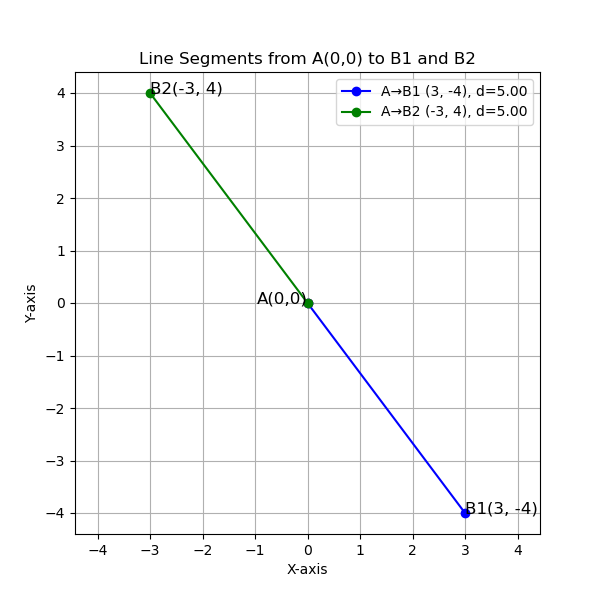
\includegraphics[width=1\columnwidth]{figs/distance.png}
    \caption{distance between two points
    }
    \label{fig:placeholder_1}
\end{figure}
\end{document}